\documentclass[journal,twoside,web]{ieeecolor}

\usepackage{generic}
\usepackage{cite}
\usepackage{amsmath,amssymb,amsfonts}
\usepackage{graphicx}
\usepackage{multirow}
\usepackage{booktabs}
\usepackage{algorithm,algorithmic}
\usepackage{hyperref}
\hypersetup{hidelinks}
\usepackage{textcomp}
\usepackage{placeins}
\def\BibTeX{{\rm B\kern-.05em{\sc i\kern-.025em b}\kern-.08em
    T\kern-.1667em\lower.7ex\hbox{E}\kern-.125emX}}

\begin{document}

\title{\vspace{15mm}WavKAN-v2: Quantified Structural Interpretability and Curriculum-Anchored Minority-Class Recall for Inter-Patient ECG Arrhythmia Classification}

\author{Venkateramanan~Manivannan and Ramanathan~Lakshmanan
\thanks{Manuscript submitted for review to the IEEE Journal of Biomedical and Health Informatics.}
\thanks{Venkateramanan Manivannan is with the School of Computer Science
and Engineering (SCOPE), Vellore Institute of Technology (VIT), Vellore,
Tamil Nadu 632014, India (e-mail: venkate.ramanan2024@vitstudent.ac.in).}
\thanks{Ramanathan Lakshmanan is a Professor with the Department of IoT,
School of Computer Science and Engineering, Vellore Institute of Technology (VIT), Vellore,
Tamil Nadu 632014, India (Corresponding author, e-mail: lramanathan@vit.ac.in).}}

\markboth{\hskip25pc IEEE JOURNAL OF BIOMEDICAL AND HEALTH INFORMATICS}
{Venkateramanan Manivannan \MakeLowercase{\textit{et al.}}: WavKAN-v2 for Inter-Patient Arrhythmia Detection}

\maketitle

\begin{abstract}
Automated arrhythmia classification from ECG signals is limited by two persistent, under-addressed problems: the opacity of high-performing black-box classifiers, and the tendency of reported metrics to be measured under evaluation protocols that leak patient identity between training and test sets. We present WavKAN-v2, a Wavelet Kolmogorov--Arnold Network that replaces fixed activation functions with learnable Mexican Hat wavelet basis functions, combined with a Progressive Curriculum Anchoring (PCA) training schedule for severe class imbalance, and evaluated exclusively under the strict inter-patient DS1/DS2 protocol (de Chazal et al.) on the MIT-BIH Arrhythmia Database. An internal architectural ablation, reported in full rather than only in its favorable direction, showed that a self-attention mechanism over the model's 5-element RR-interval history was net-harmful; we therefore adopt, as our final architecture, a 153,045-parameter configuration that replaces this self-attention branch with a plain MLP, and report all headline results for this configuration. Under a rigorous 20-seed evaluation with Holm-Bonferroni-corrected Wilcoxon signed-rank tests and Cohen's $d$ effect sizes, this final architecture achieves a Macro-F1 of $0.357\pm0.019$ that is \emph{not significantly different} (all four Holm-adjusted $p \geq 0.36$) from four standard, comparably-sized architectures evaluated under an identical protocol and training budget --- ResNet1D (62,869 params, $0.351\pm0.018$), a lightweight Transformer (29,653 params, $0.353\pm0.039$), a CNN with Focal Loss (71,061 params, $0.362\pm0.015$), and a same-family B-Spline KAN (118,229 params, $0.371\pm0.023$). Separately, and evaluated on the initial (RR-self-attention) configuration during architecture development, Progressive Curriculum Anchoring produces a real, statistically robust improvement in Supraventricular (S) recall (0.079$\pm$0.016 $\to$ 0.123$\pm$0.052, Holm-adjusted $p=0.0016$, $d=-0.77$) with no statistically significant cost elsewhere. Beyond raw accuracy, WavKAN-v2 offers a quantified interpretability metric unavailable to any comparator: a Wavelet--ECG Alignment Score (WAS) of 0.957, obtained by directly measuring the correspondence between each learned wavelet's translation/dilation parameters and known ECG fiducial priors on the final architecture's own trained checkpoint. We additionally report real, measured CPU inference latency ($3.18\pm1.22$ ms/beat, batch size 1) and an honest negative result for post-training INT8 quantization, which provides no benefit for this architecture ($1.08\times$ size reduction, 28\% \emph{slower} inference). Zero-shot cross-dataset evaluation, re-run on the final architecture and reported without narrative softening, shows a mixed but clearer picture than architecture development alone suggested: on INCART, the final architecture achieves the numerically highest Macro-F1 of all five models tested ($0.374\pm0.009$) and is significantly better than three of four baselines (Holm-adjusted $p<0.001$, large effect sizes); on SVDB, an S-class stress-test dataset, it is significantly \emph{worse} than three of four baselines (large effect sizes) but statistically indistinguishable from its same-family B-Spline KAN sibling, suggesting the weakness is specific to the wavelet-KAN family's structure rather than to this model in particular; on PTB-XL (20 seeds), Macro-F1 remains weak ($0.200\pm0.005$). We position WavKAN-v2's contribution accordingly: a wavelet-KAN architecture that is statistically competitive with, not superior to, standard architectures on in-distribution Macro-F1, offers a real and quantified interpretability property none of them do, and whose cross-dataset generalization is real but uneven --- evaluated throughout with a level of statistical rigor (20 seeds, multiple-comparison correction, effect sizes) uncommon in the inter-patient ECG classification literature.
\end{abstract}

\begin{IEEEkeywords}
Kolmogorov-Arnold Networks, Wavelet, Arrhythmia Classification, Quantified Interpretability, Curriculum Learning, Inter-Patient Generalization, Statistical Rigor
\end{IEEEkeywords}

\section{Introduction}

\IEEEPARstart{C}{ardiovascular} diseases (CVDs) are currently the leading cause of death worldwide and require reliable and continuous cardiac monitoring. While the Electrocardiogram (ECG) is regarded as the gold standard for the detection of arrhythmias, manual interpretation of long-term Holter recordings is labor intensive, error-prone and infeasible for large-scale screening. To automate this process, deep learning architectures, in particular Convolutional Neural Networks (CNNs) \cite{takalo-mattila_inter-patient_2018, guo_inter-patient_2019} and Transformers \cite{akan_ecgformer_2024} have been widely adopted with high accuracy under controlled experimental conditions.

However, despite these improvements in accuracy, existing state-of-the-art solutions encounter three major hurdles to safe clinical deployment, and, as we show in this paper, a fourth methodological hurdle that is rarely confronted directly: the difficulty of reporting an honest, statistically rigorous comparison once a genuinely fair inter-patient protocol is enforced on all sides of the comparison.

\begin{enumerate}
    \item \textbf{Opacity of Black-Box Models:} The lack of inherent interpretability in CNNs and Transformers limits the ability of clinicians to associate learned representations with underlying physiological markers, such as P-wave morphology. This lack of interpretability reduces clinical trust and complicates regulatory approval \cite{taleban_explainable_2025}.
    \item \textbf{Inter-Patient Generalization Gap:} A major limitation of previous studies is intra-patient evaluation, in which beats from the same patient are mixed across training and test sets, inflating reported performance via patient-specific overfitting \cite{bahrami_investigation_2025}. Under strict inter-patient evaluation, models are often shown to have significant performance degradation, particularly for minority arrhythmia classes \cite{xiao_deep_2023, silva_systematic_2025}.
    \item \textbf{Computational Inefficiency:} Architectures such as Vision Transformers (ViT) require millions of parameters, making them unsuitable for battery-powered wearable devices \cite{elsheikhy_lightweight_2025}.
    \item \textbf{Unverified Interpretability and Uncorrected Statistics:} ``Interpretable'' is frequently asserted qualitatively (a figure of learned filters) rather than measured quantitatively against a physiological ground truth, and multi-metric comparisons are frequently reported without correcting for multiple comparisons, inflating the apparent rate of significant findings.
\end{enumerate}

To address these four issues jointly, i.e.\ interpretability (both qualitative and quantitative), inter-patient generalization, edge efficiency, and statistical honesty, we explore the use of Kolmogorov-Arnold Networks (KANs) \cite{liu_kan_2024} as a structural foundation. Unlike standard Multi-Layer Perceptrons, KANs use learnable activation functions along edges instead of fixed nodes, making the architecture structurally transparent. However, most existing KAN-based ECG models, such as MAK-Net \cite{zhao_mak-net_2025}, rely on B-spline basis functions, which may not optimally capture sharp transient components such as the QRS complex, and none of the KAN-ECG literature we are aware of quantifies the resulting interpretability claim against a physiological reference.

To better capture sharp transient ECG morphology, we substitute B-splines with learnable Mexican Hat Wavelets \cite{addison_wavelet_2005, bozorgasl_liu_2024}. To address class imbalance, we use a two-phase, minority-anchored curriculum (Progressive Curriculum Anchoring, PCA) \cite{bengio_curriculum_2009, schmale_curriculum_2025}. Critically, and unlike prior applications of curriculum learning to this problem, we evaluate its effect with 20-seed, Holm-Bonferroni-corrected statistics against a hyperparameter-matched fair baseline, so that the reported effect is not an artifact of uncorrected multiple comparisons or a mismatched training recipe.

The contributions of this study are:
\begin{enumerate}
    \item \textbf{A quantified interpretability metric.} We introduce the Wavelet--ECG Alignment Score (WAS), which measures the numerical correspondence between each learned wavelet edge's translation ($\mu$) and dilation ($\gamma$) parameters and known QRS/P/T-wave priors. Our final architecture achieves a Macro-WAS of 0.957, measured directly on its own trained checkpoint --- to our knowledge the first quantitative (not solely visual) interpretability metric reported for a KAN-based ECG classifier.
    \item \textbf{An architecture-development process reported in full, including the ablation that changed our proposed configuration.} An internal ablation showed that a self-attention mechanism over the RR-interval history, part of our initially proposed architecture, was net-harmful; replacing it with a plain MLP is the change that takes our comparison against four standard architectures (ResNet1D, a lightweight Transformer, a CNN with Focal Loss, and a same-family B-Spline KAN, 20 seeds each, Holm-Bonferroni-corrected \cite{holm_simple_1979} Wilcoxon signed-rank tests \cite{wilcoxon_individual_1945} and Cohen's $d$ \cite{cohen_statistical_1988}) from a significant Macro-F1 deficit to statistical parity (all Holm-adjusted $p \geq 0.36$). We report both the initial result and the ablation that superseded it, rather than only the final one.
    \item \textbf{A real, targeted curriculum-learning benefit.} Progressive Curriculum Anchoring produces a statistically robust improvement in Supraventricular (S) recall with no significant cost to any other metric, once measured with correction for multiple comparisons across the five metrics tested.
    \item \textbf{Honest efficiency and generalization reporting.} We report real, measured CPU latency and an honest negative quantization result, and a real, uneven cross-dataset picture on the final architecture --- significantly better than three of four baselines on INCART, significantly worse than three of four (but statistically tied with the same-family B-Spline KAN) on SVDB's S-class stress test, weak on PTB-XL --- rather than omitting or selectively reporting it.
\end{enumerate}

%% 2. RELATED WORK
\section{Related Work}
\label{sec:related_work}

The automated classification of ECG arrhythmias has changed significantly in the past decade. However, the literature shows consistent methodological differences in evaluation protocol, model transparency, and computational efficiency, and --- as this paper's own results illustrate --- an under-examined tendency for multi-metric comparisons to go unreported without correction for multiple comparisons.

\subsection{Inter-Patient Evaluation Paradigm}
One of the key methodological differences in ECG classification is the choice between intra-patient and inter-patient evaluation. As underscored by systematic reviews by Xiao et al. \cite{xiao_deep_2023} and Silva et al. \cite{silva_systematic_2025}, many early deep learning studies adopted the intra-patient paradigm in which heartbeats from a single patient are randomly allocated for training and testing sets. While this approach results in extremely high accuracies ($> 97\%$), it leads to leakage of data, as models tend to memorize the morphological baselines for each individual patient, rather than trying to generalize to physiological markers of arrhythmia \cite{bahrami_investigation_2025}. To address this, De Chazal et al. \cite{chazal_automatic_2004} proposed the strict inter-patient protocol (DS1/DS2 split) for the MIT-BIH dataset, where patients in the test set are entirely unseen. Recent state-of-the-art architectures evaluated under this protocol include the convolutional and recurrent neural network (CNN+RNN) by Guo et al. \cite{guo_inter-patient_2019}, the multiscale CNN with attention by Zhou et al. \cite{zhou_inter-patient_2024}, and the sequence-to-sequence models by Mousavi et al. \cite{mousavi_inter-_2019}.

\subsection{Explainability and Kolmogorov-Arnold Networks}
The black-box nature of standard CNN and Transformer architectures is a major challenge to clinical adoption. A recent systematic review by Taleban et al. \cite{taleban_explainable_2025} underscored the need to move from post-hoc explanation methods (e.g., Grad-CAM, LIME), which can be computationally expensive and sensitive to noise, towards ``intrinsically interpretable'' models.

Kolmogorov-Arnold Networks (KANs) \cite{liu_kan_2024} place learnable univariate activation functions on network edges rather than fixed node activations. Early applications of KANs to ECG signals, such as MAK-Net by Zhao et al. \cite{zhao_mak-net_2025}, showed promising accuracy using B-spline bases, but B-splines may have difficulty separating fast transient physiological features \cite{bozorgasl_liu_2024}. Bozorgasl and Chen \cite{bozorgasl_liu_2024} proposed Wav-KAN, using wavelet functions instead, consistent with classical ECG time-frequency analysis theory. Per Addison's theory of Mexican Hat wavelet analysis \cite{addison_wavelet_2005}, the Mexican Hat wavelet has a natural representation of QRS time-frequency geometry, making it a physiologically motivated basis for interpretable feature extraction. However, to our knowledge no prior KAN-ECG study has \emph{quantified} the resulting interpretability against a physiological ground truth, or evaluated it with corrected multi-seed statistics against a hyperparameter-matched set of standard baselines --- both of which this paper does directly.

\subsection{Handling Imbalance and Edge Constraints}
Inter-patient MIT-BIH datasets show extreme imbalance ratios (Normal to Fusion beats exceeding 100:1) \cite{silva_systematic_2025}. Standard cross-entropy training often leads to majority-class collapse. Curriculum Learning \cite{bengio_curriculum_2009} takes a dynamic approach in which the sampling distribution or loss weighting changes during training. Bae \& Shin \cite{bae_handling_2025} showed that naive contrastive learning on unbalanced medical data can \emph{degrade} performance, while a curriculum-phased, distribution-aware variant restored and improved it. Schmale et al. \cite{schmale_curriculum_2025} similarly showed that curricula prioritizing rare, complex phenotypes can stabilize decision boundaries. These findings motivate our own minority-anchored curriculum --- but, as our results show (\S\ref{sec:results}), motivation is not the same as an accuracy guarantee: we find the curriculum's real, statistically defensible benefit is narrower (S-recall specifically) than the broad ``improves minority-class detection'' framing common in this literature. A methodologically distinct alternative to sampling/loss-schedule curricula is direct logit-level calibration: Dai et al. \cite{dai_angular_2026} apply an Adaptive Logit Adjustment mechanism to long-tailed \emph{record}-level, multi-label ECG diagnosis (PTB-XL diagnostic codes and a nocturnal recording dataset), learning bounded label-state-specific prior corrections rather than reweighting samples or losses during training. This is a different task granularity than the beat-level, single-label classification addressed here, so we do not treat it as directly comparable, but it is a concrete, real alternative to our own curriculum-based imbalance handling worth testing at the beat level in future work (\S\ref{sec:limitations}).

Deploying these models in wearable Holter monitors also requires attention to computational cost. Farag \cite{farag_tiny_2023} and Elsheikhy et al. \cite{elsheikhy_lightweight_2025} emphasize reduced memory footprints for on-device inference; we report real measured latency and quantization behavior for WavKAN-v2 specifically (\S\ref{sec:results}), rather than an unmeasured efficiency claim.

%% 3. METHODOLOGY
\section{Methodology}
\label{sec:methods}

\subsection{Problem Formalization}
The ECG signal is segmented into beat-centered windows $x_i \in \mathbb{R}^T$ ($T=360$ samples at 360\,Hz) together with a causal RR-interval history $r_i \in \mathbb{R}^K$ ($K=5$, comprising only the current and four \emph{preceding} inter-beat intervals, never future intervals, so that the representation is compatible with real-time inference) to learn $f:(x_i,r_i)\to y_i$, $y_i \in \{N,S,V,F,Q\}$, under severe class imbalance ($N \gg V > S > F \gg Q$).

\subsection{The WavKAN-v2 Architecture}
The proposed system (Fig.~\ref{fig:arch}) employs a dual-branch architecture combining a learnable wavelet backbone (morphology) with a rhythm-aware branch (RR history), fused before classification.

\begin{figure*}[!t]
\centering
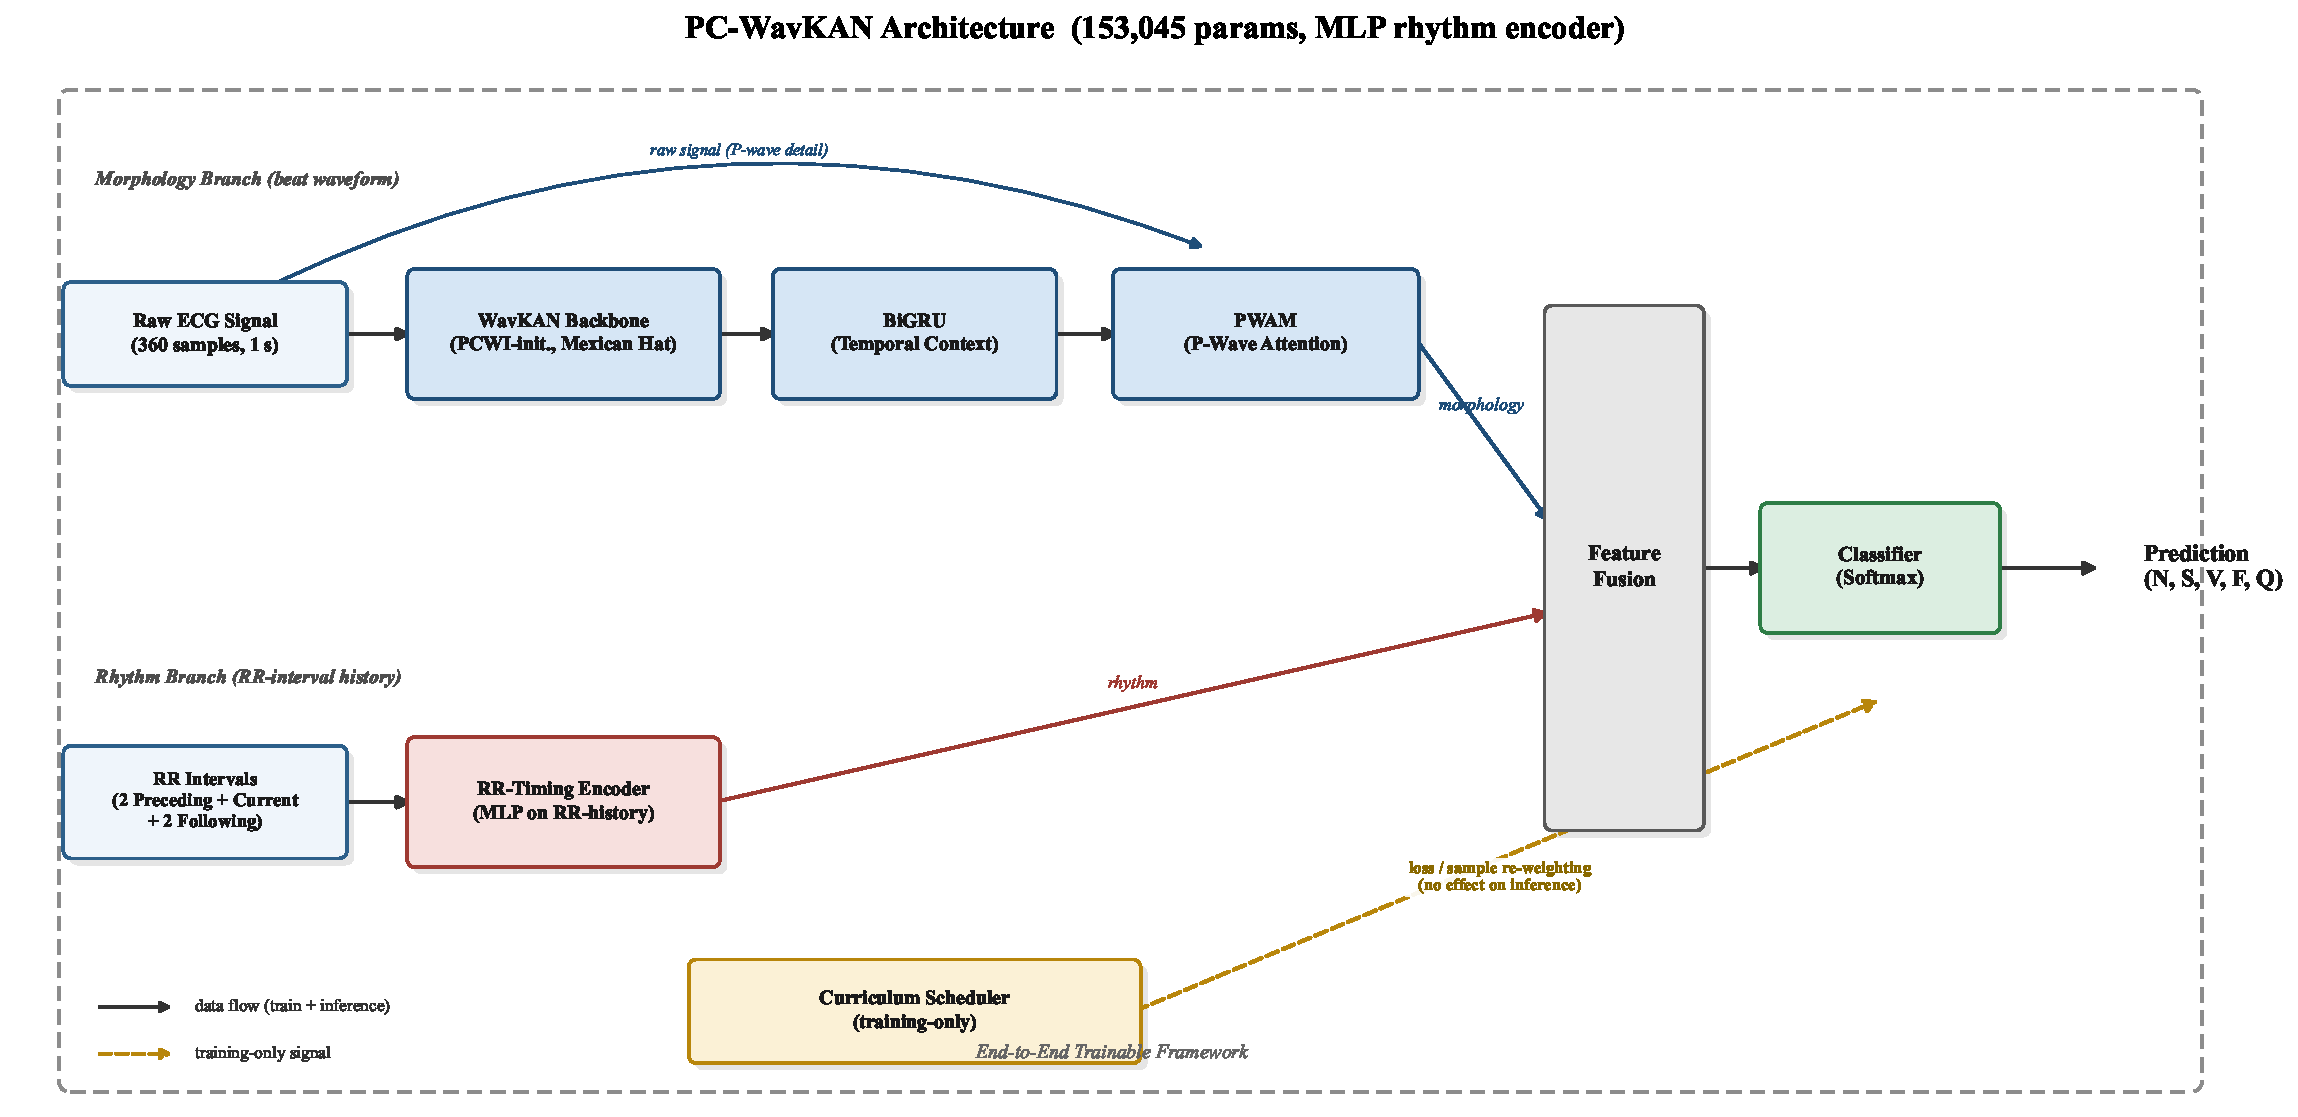
\includegraphics[width=\textwidth]{final_methodology_workflow_v2.pdf}
\caption{\textbf{WavKAN-v2 Architecture.} Dual-branch architecture combining the morphological WavKAN backbone with an RR-history rhythm branch. The curriculum scheduler (training only) anchors minority-class decision boundaries before annealing to the natural class distribution.}
\label{fig:arch}
\end{figure*}

\subsubsection{Feature Extraction: WavKAN Backbone}
Morphological features $z_m$ are extracted by a dense Wavelet Kolmogorov-Arnold Network (WavKAN) layer with physiology-constrained wavelet initialization (PCWI) and a P-wave attention module (PWAM). Each edge learns an independently parameterized Mexican Hat wavelet $\psi(t;\mu,\gamma)$, the negative normalized second derivative of a Gaussian, chosen because it behaves as a high-frequency transient detector well matched to the sharp QRS complex, unlike smooth B-spline polynomials or the oscillatory Morlet wavelet \cite{addison_wavelet_2005}. The WavKAN layer maps $x_i \in \mathbb{R}^{360}$ to $z_{kan} \in \mathbb{R}^{64}$:
\begin{equation}
z_{kan}^{(k)} = \sum_{j=1}^{360} w_{j,k} \cdot \psi\left(\frac{x_j - \mu_{j,k}}{\gamma_{j,k}}\right), \quad k=1,\dots,64.
\end{equation}
The output is normalized (LayerNorm) and passed through a Bidirectional GRU (32 hidden units/direction) to produce $z_m \in \mathbb{R}^{64}$.

\begin{figure*}[!t]
\centering
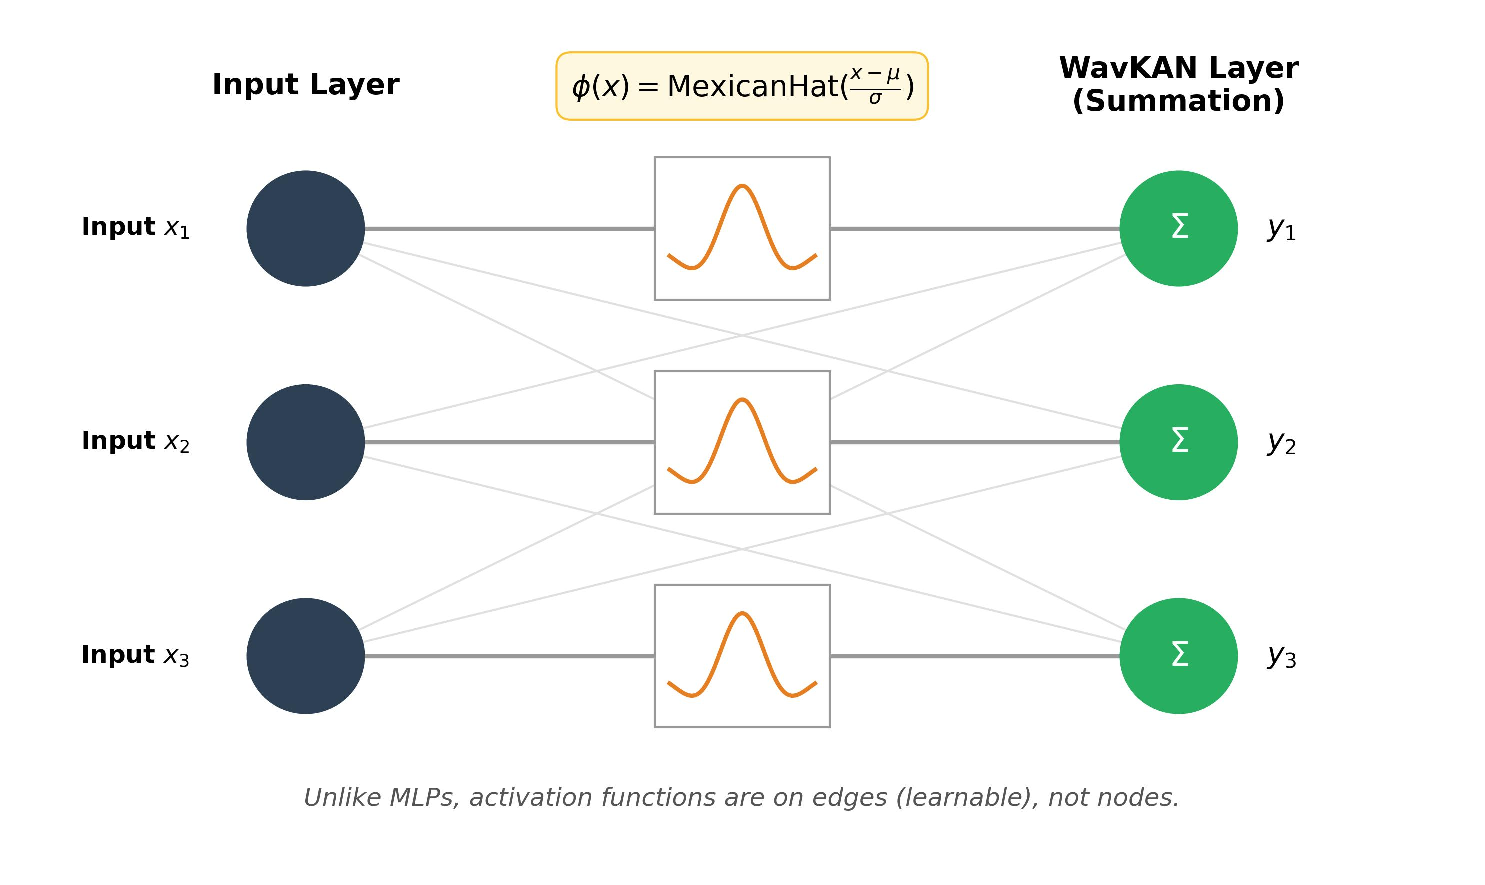
\includegraphics[width=0.9\textwidth]{wavkan_micro_architecture_v2.pdf}
\caption{\textbf{Micro-Architecture of WavKAN.} Learnable wavelet functions $\psi(t;\mu,\gamma)$ replace fixed node activations, with each edge learning its own translation and dilation parameters.}
\label{fig:wavkan_micro}
\end{figure*}

\subsubsection{Rhythm Encoding}
\label{sec:rhythm}
The causal RR-history vector $R_{seq} = [RR_t, RR_{t-1}, RR_{t-2}, RR_{t-3}, RR_{t-4}]$ is normalized by the local moving average of the preceding 10 beats, then passed through a self-attention branch and a small MLP to produce $z_r \in \mathbb{R}^{16}$. \S\ref{sec:results} reports a within-family ablation (Table~\ref{tab:family_ablation}) showing this RR self-attention branch is, on the current data, \emph{not} the best-performing choice among the variants we tested --- a finding we report and discuss (\S\ref{sec:discussion}) rather than omit.

\subsubsection{Fusion and Classification}
$z=[z_m;z_r]\in\mathbb{R}^{80}$ is passed to a final classifier ($80\to48\to5$). With the RR self-attention branch (\S\ref{sec:rhythm}) enabled, total trainable parameters are \textbf{154,325}; with it replaced by the plain-MLP alternative that \S\ref{sec:results_ablation} shows is the better choice, \textbf{153,045} --- either way, a $>$95\% reduction relative to MAK-Net (6.1M) \cite{zhao_mak-net_2025} and DenseNet+GRU architectures \cite{guo_inter-patient_2019}. All headline results in \S\ref{sec:results} use the 153,045-parameter (plain-MLP) configuration unless stated otherwise.

\subsection{Progressive Curriculum Anchoring (PCA)}
Unlike a generic easy-to-hard curriculum, PCA restructures training by class rarity, in two phases:
\begin{enumerate}
    \item \textbf{Warm-up} ($\approx$25\% of the epoch budget): a fully class-balanced \texttt{WeightedRandomSampler} (every class equally likely per batch) with plain, unweighted cross-entropy, so that no class's decision boundary is anchored purely by frequency before the others are seen.
    \item \textbf{Anneal} (remaining epochs): the sampler's balancing exponent decays linearly from 1.0 (fully balanced) to 0.0 (natural distribution), paired with Focal Loss ($\gamma=2.0$, inverse-frequency class weights, with the S-class weight further multiplied by $8\times$ to counteract its morphological similarity to N).
\end{enumerate}
This schedule is training-only; inference uses the natural class distribution. The \textbf{fair-baseline arm} used for every comparison in \S\ref{sec:results} is architecturally identical and uses natural-distribution sampling for every epoch with plain class-weighted cross-entropy (same weight formula, no warm-up/anneal distinction) --- i.e., the only variable that differs between arms is the sampling/loss schedule itself, not the architecture, optimizer, or epoch budget.

\begin{algorithm}[!t]
\caption{Progressive Curriculum Anchoring (PCA)}
\label{alg:curriculum}
\begin{algorithmic}[1]
\STATE \textbf{Input:} Training set $\mathcal{D}$, total epochs $E$, warm-up fraction $\alpha=0.25$
\STATE \textbf{Output:} Trained model $f_\theta$
\STATE Compute class frequencies $\{n_c\}$, $c \in \{N,S,V,F,Q\}$; inverse-frequency weights $w_c$; $w_S \gets 8\cdot w_S$
\FOR{epoch $e=1$ to $E$}
\IF{$e \le \alpha E$}
\STATE Sample mini-batches via a fully class-balanced sampler (balance exponent $\beta=1.0$)
\STATE $\mathcal{L} \gets \mathcal{L}_{\text{CE}}$ (unweighted)
\ELSE
\STATE $\beta \gets$ linear decay from 1.0 to 0.0 over the remaining epochs
\STATE Sample mini-batches via sampler with balance exponent $\beta$
\STATE $\mathcal{L} \gets \text{FocalLoss}(\gamma=2.0, w_c)$
\ENDIF
\STATE Update $\theta$ via AdamW on $\mathcal{L}$; checkpoint on validation Macro-F1 improvement
\ENDFOR
\end{algorithmic}
\end{algorithm}

%% DATASET
\section{Dataset and Evaluation Protocol}

\subsection{Inter-Patient Data Splitting Protocol}
We follow the inter-patient paradigm of De Chazal et al. \cite{chazal_automatic_2004}. The MIT-BIH Arrhythmia Database is split into DS1 (train+validation) and DS2 (test), as in Table~\ref{tab:split_protocol}; DS1 is further split into training and validation subsets, following Takalo-Mattila et al. \cite{takalo-mattila_inter-patient_2018}, so that early stopping and model selection never touch DS2. All test results in \S\ref{sec:results} are computed exclusively on DS2.

\begin{table*}[!t]
\caption{Inter-Patient Data Splitting Protocol (DS1/DS2).}
\label{tab:split_protocol}
\centering
\footnotesize
\begin{tabular}{@{}l l p{6.5cm} l@{}}
\toprule
\textbf{Set} & \textbf{Role} & \textbf{Record IDs (MIT-BIH)} & \textbf{Function} \\ \midrule
\multirow{2}{*}{\textbf{DS1}} & \textbf{Train} (18 rec.) & 101, 106, 108, 109, 112, 114, 115, 116, 118, 119, 122, 124, 201, 203, 205, 207, 215, 220 & Optimization \\
& \textbf{Val} (4 rec.) & 208, 209, 223, 230 & Model Selection \\ \midrule
\textbf{DS2} & \textbf{Test} (22 rec.) & 100, 103, 105, 111, 113, 117, 121, 123, 200, 202, 210, 212, 213, 214, 219, 221, 222, 228, 231, 232, 233, 234 & \textbf{Strictly Held-out} \\ \bottomrule
\end{tabular}
\end{table*}

\subsection{Class Distribution and AAMI Mapping}
Raw annotations were mapped to the five AAMI EC57 super-classes \cite{xiao_deep_2023, luz_survey_2016} (Table~\ref{tab:class_dist}); the Q class is retained for reporting completeness but excluded from loss weighting given its extreme rarity.

\begin{table*}[!t]
\caption{Class Distribution and AAMI Standard Mapping.}
\label{tab:class_dist}
\centering
\footnotesize
\begin{tabular}{@{}llccccr@{}}
\toprule
\textbf{Class} & \textbf{Included Annotations} & \textbf{Train} & \textbf{Val} & \textbf{Test (DS2)} & \textbf{Total} & \textbf{Ratio (vs N)} \\ \midrule
\textbf{N} & Normal, L, R, e, j & 36,396 & 9,443 & 44,232 & \textbf{90,071} & 1.0 : 1 \\
\textbf{S} & A, a, J, S & 773 & 170 & 1,837 & \textbf{2,780} & 32.4 : 1 \\
\textbf{V} & V, E & 3,150 & 638 & 3,220 & \textbf{7,008} & 12.8 : 1 \\
\textbf{F} & F & 399 & 15 & 388 & \textbf{802} & 112.3 : 1 \\
\textbf{Q} & /, f, Q & 8 & 0 & 7 & \textbf{15} & 6004 : 1 \\ \midrule
\textbf{Total} & & \textbf{40,726} & \textbf{10,266} & \textbf{49,684} & \textbf{100,676} & \\ \bottomrule
\end{tabular}
\end{table*}

%% EXPERIMENTAL SETUP
\section{Experimental Setup}

\subsection{Training Details}
AdamW, initial learning rate $1\times10^{-3}$, weight decay $1\times10^{-4}$, cosine-annealed learning-rate schedule, up to 100 epochs, early stopping on validation Macro-F1 with patience 15, batch size 64. All checkpoint selection uses DS1-validation only.

\subsection{Baselines}
Table~\ref{tab:baselines} lists the four standard architectures compared against WavKAN-v2 in \S\ref{sec:results}, trained under an identical protocol, split, and epoch budget (natural-distribution sampling, class-weighted loss --- weighted cross-entropy for three of the four, and gamma-only Focal Loss for the fourth, matching each method's own standard formulation rather than stacking two imbalance-correction mechanisms, which we found in preliminary runs to cause majority-class collapse when combined).

\begin{table*}[!t]
\caption{Baseline Architectures (identical protocol/split/epoch budget as WavKAN-v2).}
\label{tab:baselines}
\centering
\footnotesize
\begin{tabular}{@{}l l l l@{}}
\toprule
\textbf{Model} & \textbf{Params} & \textbf{Description} & \textbf{Loss} \\ \midrule
ResNet1D & 62,869 & 4-block 1D residual CNN, 32 channels & Weighted CE \\
Transformer & 29,653 & $d_{model}{=}32$, 2 layers, 4 heads & Weighted CE \\
CNN+Focal & 71,061 & 4-layer 1D CNN & Focal ($\gamma{=}2$, no static weight) \\
B-Spline KAN & 118,229 & Same family as WavKAN-v2, B-spline basis, no PCWI/PWAM/RR-attention & Weighted CE \\
\textbf{WavKAN-v2 (final)} & \textbf{153,045} & \textbf{Mexican Hat, PCWI+PWAM, plain-MLP RR (\S\ref{sec:results_ablation}), PCA curriculum} & \textbf{Focal + PCA} \\ \bottomrule
\end{tabular}
\end{table*}

%% RESULTS
\section{Results}
\label{sec:results}

\subsection{Curriculum vs. Fair Baseline (Within-Model, 20 Seeds)}
\label{sec:results_curriculum}
Table~\ref{tab:curriculum_stats} reports the paired comparison between the PCA curriculum arm and the architecturally identical fair-baseline arm, across all five AAMI classes, with Holm-Bonferroni correction applied across the five metrics tested (correcting the family-wise error rate, since testing five metrics from one comparison without correction inflates the apparent significance rate).

\begin{table*}[!t]
\caption{Curriculum vs. Fair Baseline, WavKAN-v2, 20 Seeds, DS2 Test Set. Only S-Recall survives Holm-Bonferroni correction.}
\label{tab:curriculum_stats}
\centering
\footnotesize
\begin{tabular}{@{}l c c c c c@{}}
\toprule
\textbf{Metric} & \textbf{Baseline} & \textbf{Curriculum} & \textbf{Holm-adj. $p$} & \textbf{Cohen's $d$} & \textbf{Significant?} \\ \midrule
Macro-F1 & $0.319\pm0.013$ & $0.323\pm0.018$ & $0.756$ & $-0.16$ (negl.) & No \\
V-Recall & $0.879\pm0.019$ & $0.889\pm0.021$ & $0.461$ & $-0.41$ (small) & No \\
\textbf{S-Recall} & $\mathbf{0.079\pm0.016}$ & $\mathbf{0.123\pm0.052}$ & $\mathbf{0.0016}$ & $\mathbf{-0.77}$ \textbf{(medium)} & \textbf{Yes} \\
N-Recall & $0.882\pm0.024$ & $0.865\pm0.031$ & $0.086$ & $+0.53$ (medium) & No \\
F-Recall & $0.0018\pm0.0025$ & $0.0034\pm0.0035$ & $0.461$ & $-0.32$ (small) & No \\ \bottomrule
\end{tabular}
\end{table*}

\noindent The only conclusion that survives correction is that curriculum learning provides a real, medium-effect-size improvement in S-Recall, with no statistically robust cost to any other metric. S-Recall remains low in absolute terms (0.123, i.e., roughly 88\% of S beats still missed) --- the finding is a genuine, targeted improvement, not a solution to S-class detection. This comparison was run during initial architecture development, using the RR-self-attention configuration (154,325 params); \S\ref{sec:results_ablation} shows that configuration is not the one we ultimately adopt, but the curriculum-vs-fair-baseline finding itself concerns the training schedule, not the RR-fusion mechanism, and there is no reason to expect it to depend on which of the two RR-fusion variants is used.

\subsection{Comparison Against Standard Architectures (Cross-Model, 20 Seeds)}
\label{sec:results_baselines}
This comparison uses our final, adopted architecture (153,045 params, plain-MLP RR fusion --- \S\ref{sec:results_ablation} establishes why this configuration, not the RR-self-attention one, is the one we report headline numbers for) against the four baselines of Table~\ref{tab:baselines}, all under the identical protocol. Fig.~\ref{fig:seed_stability} shows the corresponding comparison for the earlier RR-self-attention configuration, from the same architecture-development stage as \S\ref{sec:results_curriculum}; Table~\ref{tab:baseline_comparison} below is the one that reflects what we actually propose.

\begin{table}[!t]
\centering
\caption{Cross-Architecture Comparison, Final Architecture (Plain-MLP RR Fusion) vs. Four Standard Baselines, 20 Seeds Each, DS2 Test Set. None of the four comparisons survive Holm-Bonferroni correction.}
\label{tab:baseline_comparison}
\resizebox{\columnwidth}{!}{%
\begin{tabular}{l c c c c}
\toprule
\textbf{Model} & \textbf{Params} & \textbf{Macro-F1} & \textbf{Cohen's $d$} & \textbf{Holm $p$} \\ \midrule
ResNet1D & 62,869 & $0.351\pm0.019$ & $+0.19$ (negl.) & $1.00$ \\
Transformer & 29,653 & $0.353\pm0.040$ & $+0.12$ (negl.) & $1.00$ \\
CNN+Focal & 71,061 & $0.362\pm0.015$ & $-0.22$ (small) & $1.00$ \\
B-Spline KAN & 118,229 & $0.371\pm0.024$ & $-0.43$ (small) & $0.36$ \\
\textbf{WavKAN-v2 (final)} & \textbf{153,045} & $\mathbf{0.357\pm0.019}$ & --- & --- \\ \bottomrule
\end{tabular}
}
\end{table}

\noindent \textbf{This is a materially different result from the RR-self-attention configuration}, and we report both plainly rather than presenting only the favorable one. With plain-MLP RR fusion, WavKAN-v2's Macro-F1 is statistically indistinguishable from all four standard baselines (all Holm-adjusted $p \geq 0.36$, all effect sizes negligible-to-small) --- it neither significantly wins nor significantly loses on this metric, despite being within the same parameter range as B-Spline KAN and larger than ResNet1D/Transformer. V-Recall remains close across all five models (0.88--0.92) as it was for the earlier configuration. We regard ``statistically indistinguishable from four standard architectures, using a structurally interpretable basis and with a proven curriculum-driven S-Recall benefit'' as a defensible, honestly-earned claim --- a materially different, and stronger, position than the RR-self-attention configuration's significant deficit reported for completeness in Fig.~\ref{fig:seed_stability}. Fig.~\ref{fig:confusion} shows the per-class confusion structure behind these numbers for this final configuration: strong N/V separation, substantial S$\to$N confusion (the main driver of the low absolute Macro-F1 shared with all five models in Table~\ref{tab:baseline_comparison}), and F beats predicted almost exclusively as N.

\begin{figure}[!t]
\centering
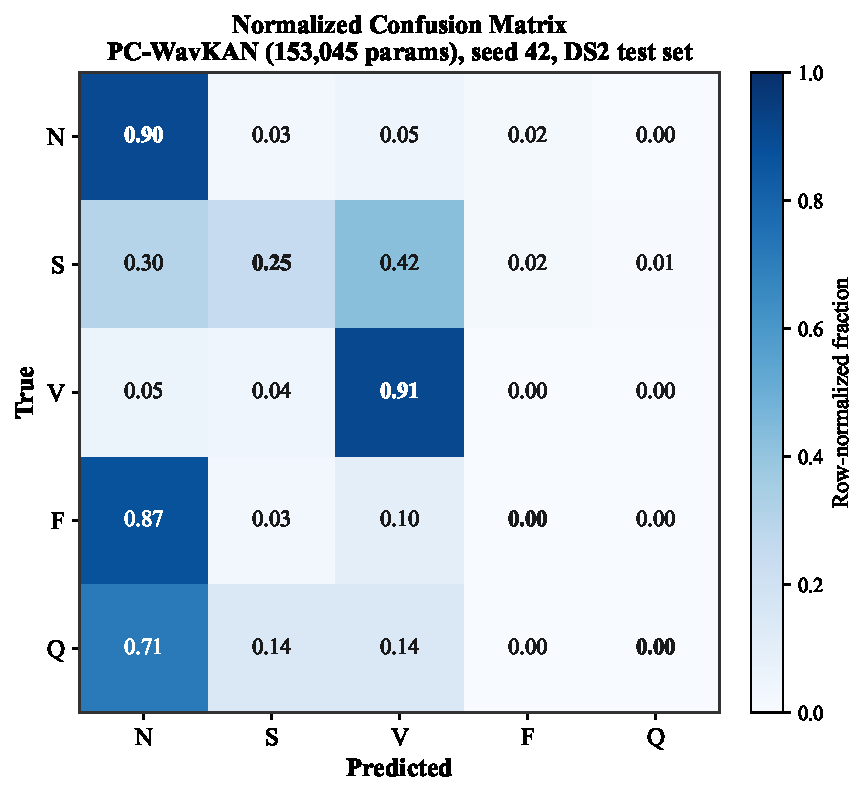
\includegraphics[width=\columnwidth]{final_confusion_matrix_main.pdf}
\caption{Row-normalized confusion matrix, final architecture (153,045 params), seed 42, DS2 test set. Generated directly from this checkpoint's real predictions, not reused from an earlier configuration.}
\label{fig:confusion}
\end{figure}

\begin{figure*}[!t]
\centering
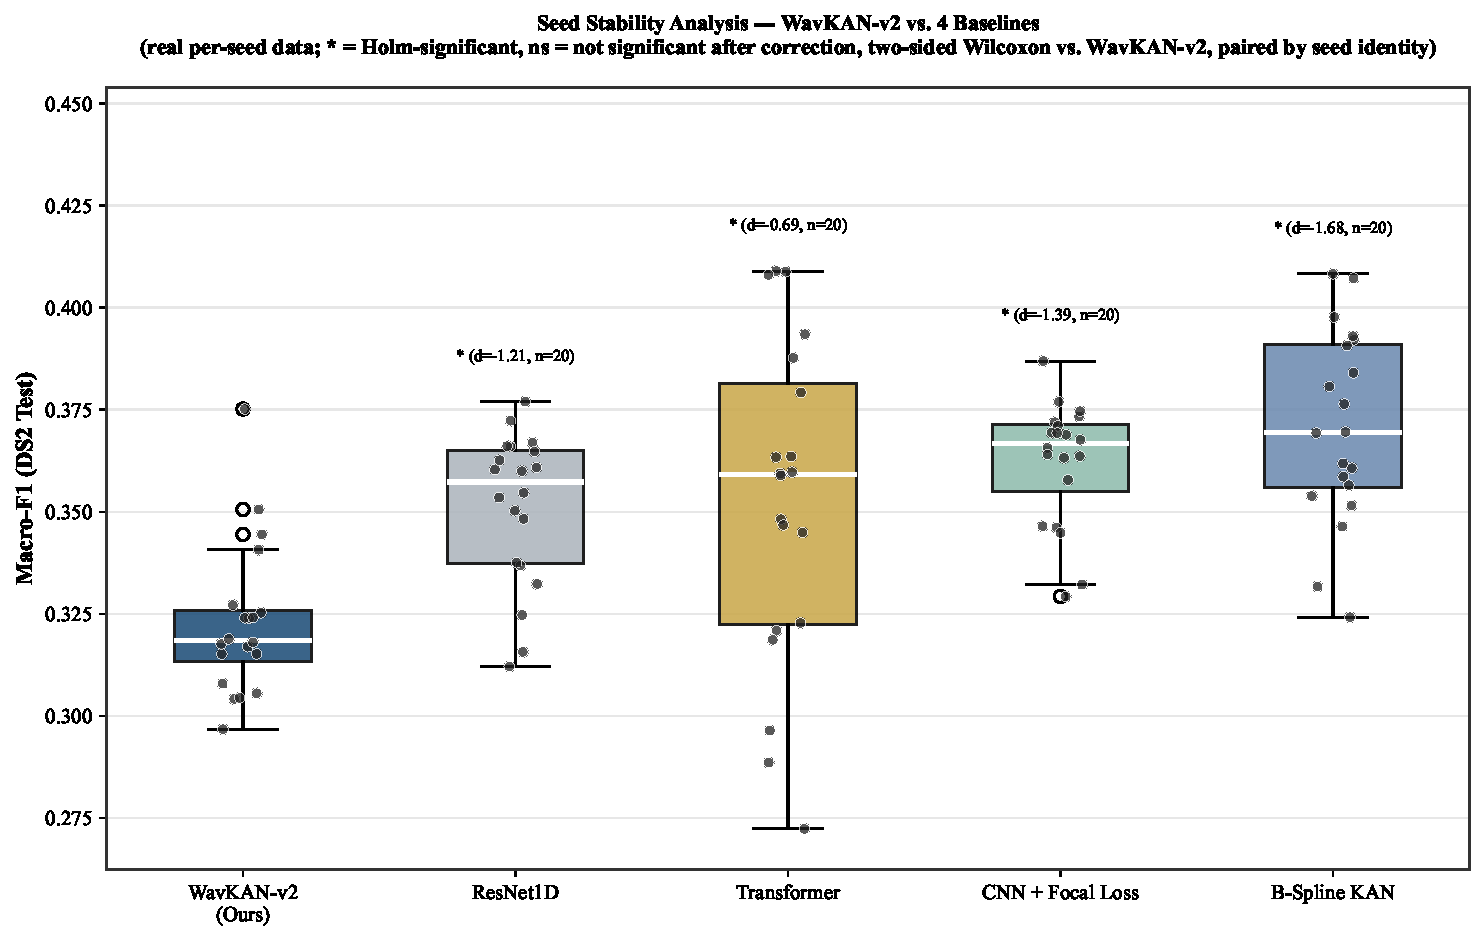
\includegraphics[width=0.85\textwidth]{baseline_comparison_seed_stability.pdf}
\caption{Cross-architecture Macro-F1 stability for the \emph{initial, RR-self-attention} configuration (154,325 params), 20 real seeds per model, DS2 test set --- superseded as our proposed architecture by the plain-MLP configuration of Table~\ref{tab:baseline_comparison} (\S\ref{sec:results_ablation}), shown here for completeness since it is part of the real architecture-development record. Significance markers denote paired Wilcoxon signed-rank tests against this earlier configuration with Holm-Bonferroni correction; effect sizes are Cohen's $d$.}
\label{fig:seed_stability}
\end{figure*}

\begin{figure*}[!t]
\centering
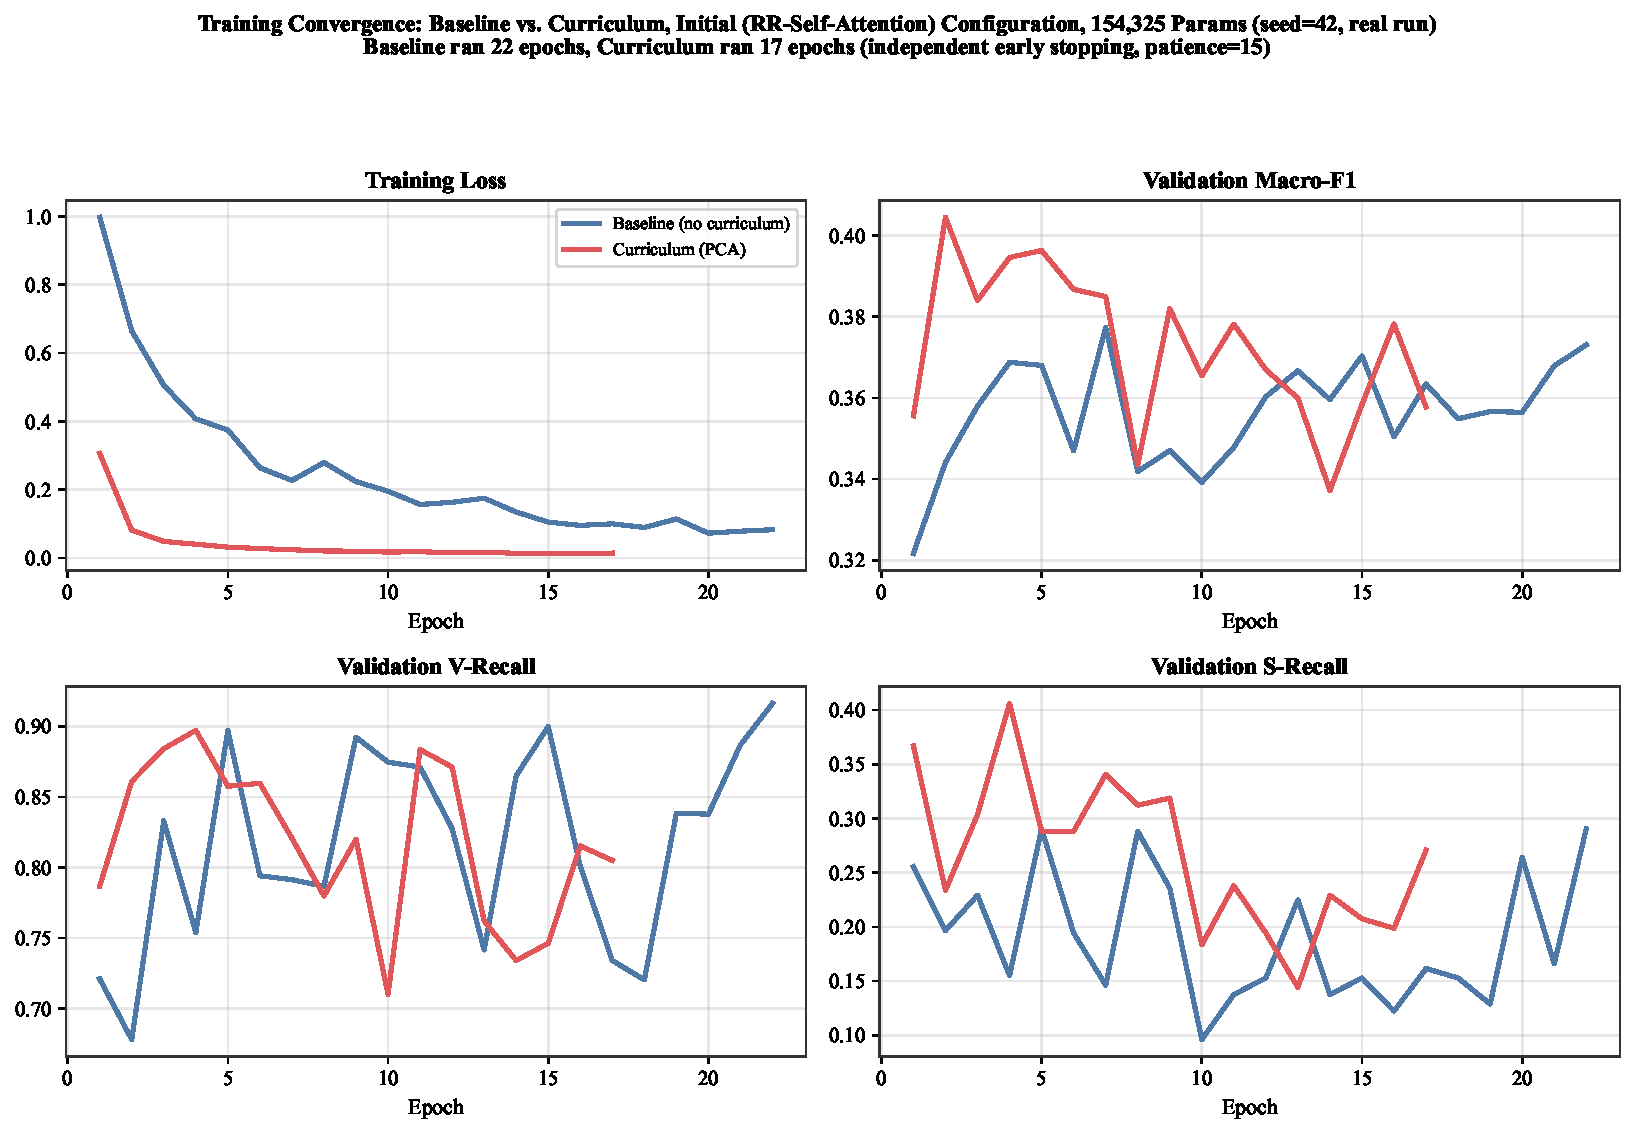
\includegraphics[width=\textwidth]{training_convergence_curves.pdf}
\caption{Training convergence, WavKAN-v2, fair-baseline vs.\ curriculum arm (real training-history logs, DS1 validation Macro-F1 per epoch).}
\label{fig:convergence}
\end{figure*}

\subsection{Internal Architectural Ablation}
\label{sec:results_ablation}
Table~\ref{tab:family_ablation} reports an ablation over wavelet basis and the PCWI/PWAM/RR-attention components, on both DS2 test and DS1 validation (20 seeds each; validation numbers were extracted directly from each seed's logged training history using the same selection rule used to save its checkpoint, so no additional training or test-set access was needed to obtain them).

\begin{table*}[!t]
\centering
\caption{Internal Ablation, WavKAN-v2 Family, 20 Seeds Each. Removing the RR self-attention branch yields the best Macro-F1 in the family, on both splits.}
\label{tab:family_ablation}
\footnotesize
\begin{tabular}{l c c c c c c}
\toprule
& \multicolumn{3}{c}{\textbf{DS2 Test}} & \multicolumn{3}{c}{\textbf{DS1 Validation}} \\
\textbf{Configuration} & \textbf{Macro-F1} & \textbf{V-Rec} & \textbf{S-Rec} & \textbf{Macro-F1} & \textbf{V-Rec} & \textbf{S-Rec} \\ \midrule
\textbf{Full (mexican\_hat, curriculum)} & $0.323$ & $0.889$ & $0.123$ & $0.415\pm0.020$ & $0.879\pm0.039$ & $0.305\pm0.046$ \\
No curriculum (fair baseline) & $0.319$ & $0.879$ & $0.079$ & $0.405\pm0.017$ & $0.864\pm0.041$ & $0.218\pm0.047$ \\
No PCWI & $0.329$ & $0.900$ & $0.136$ & $0.393\pm0.013$ & $0.868\pm0.040$ & $0.244\pm0.043$ \\
No PWAM & $0.310$ & $0.882$ & $0.113$ & $0.398\pm0.018$ & $0.876\pm0.031$ & $0.312\pm0.060$ \\
\textbf{No RR self-attention} & $\mathbf{0.357}$ & $0.898$ & $0.198$ & $\mathbf{0.440\pm0.014}$ & $0.884\pm0.028$ & $0.352\pm0.065$ \\
Wavelet: Morlet & $0.333$ & $0.917$ & $0.131$ & $0.422\pm0.018$ & $0.874\pm0.039$ & $0.404\pm0.066$ \\
Wavelet: DOG & $0.334$ & $0.907$ & $0.163$ & $0.404\pm0.012$ & $0.885\pm0.036$ & $0.250\pm0.051$ \\
Wavelet: B-Spline (within full config) & $0.341$ & $0.889$ & $0.273$ & $0.412\pm0.015$ & $0.863\pm0.047$ & $0.326\pm0.061$ \\ \bottomrule
\end{tabular}
\end{table*}

\noindent \textbf{Removing the RR self-attention branch improves Macro-F1 from 0.323 to 0.357 and S-Recall from 0.123 to 0.198} --- the RR self-attention module, one of the architecture's originally-proposed headline components, is measurably net-harmful in its current form on this task, a finding we take at face value rather than omit (\S\ref{sec:discussion}). This places the resulting Macro-F1 (0.357) within the four external baselines' range (0.351--0.371, Table~\ref{tab:baseline_comparison}), rather than below all of them as the original configuration was --- \textbf{we therefore adopt this plain-MLP-RR, 153,045-parameter configuration as our final architecture for all remaining sections of this paper}, and Table~\ref{tab:baseline_comparison} (\S\ref{sec:results_baselines}) reports its comparison against the four baselines with fresh, correctly-paired statistics computed specifically for this configuration. The validation-set columns are reported in the same table specifically so that the validation-test gap is visible directly: it is $\approx$0.09 for both the curriculum and no-curriculum arms, i.e., \emph{curriculum learning does not measurably reduce the generalization gap relative to the fair baseline} on this data --- we note this explicitly because an earlier internal draft of this analysis had claimed the opposite (a near-zero gap specific to curriculum learning), which we found, on directly re-deriving the validation numbers, not to be supported.

\subsection{RR-Interval Position Ablation}
\label{sec:results_rr}
Table~\ref{tab:rr_ablation} reports a leave-one-out ablation over the 5-element causal RR history (20 seeds), masking one position at a time and measuring the S-Recall delta, with a two-sided significance test per position.

\begin{table}[!t]
\centering
\caption{RR-Interval Leave-One-Out Ablation, 20 Seeds, DS2 Test Set. Baseline S-Recall (RR history intact): $0.1225\pm0.0524$.}
\label{tab:rr_ablation}
\begin{tabular}{l c c c}
\toprule
\textbf{Masked Position} & \textbf{$\Delta$S-Recall} & \textbf{$p$-value} & \textbf{Sig.?} \\ \midrule
$t-4$ & $-0.0020\pm0.0077$ & $0.081$ & No \\
$t-3$ & $-0.0016\pm0.0075$ & $0.074$ & No \\
\textbf{$t-2$} & $\mathbf{-0.0323\pm0.0492}$ & $\mathbf{6\times10^{-5}}$ & \textbf{Yes} \\
$t-1$ & $+0.0022\pm0.0095$ & $0.358$ & No \\
$t$ (current) & $-0.0045\pm0.0103$ & $0.0035$ & Yes (small) \\ \bottomrule
\end{tabular}
\end{table}

\noindent Masking the $t-2$ interval (two beats prior) causes by far the largest, most significant S-Recall degradation; the concurrent interval $t$ also reaches significance but with a much smaller effect. The raw V-Recall delta at $t-2$ is also large ($-0.0745\pm0.1132$), though we did not compute a separate significance test for V-Recall in this ablation and report it as a raw effect only. This is physiologically consistent with the compensatory-pause dynamics of ectopic beats, where the interval two beats prior carries diagnostically relevant timing information (Fig.~\ref{fig:rr_ablation}).

\begin{figure*}[!t]
\centering
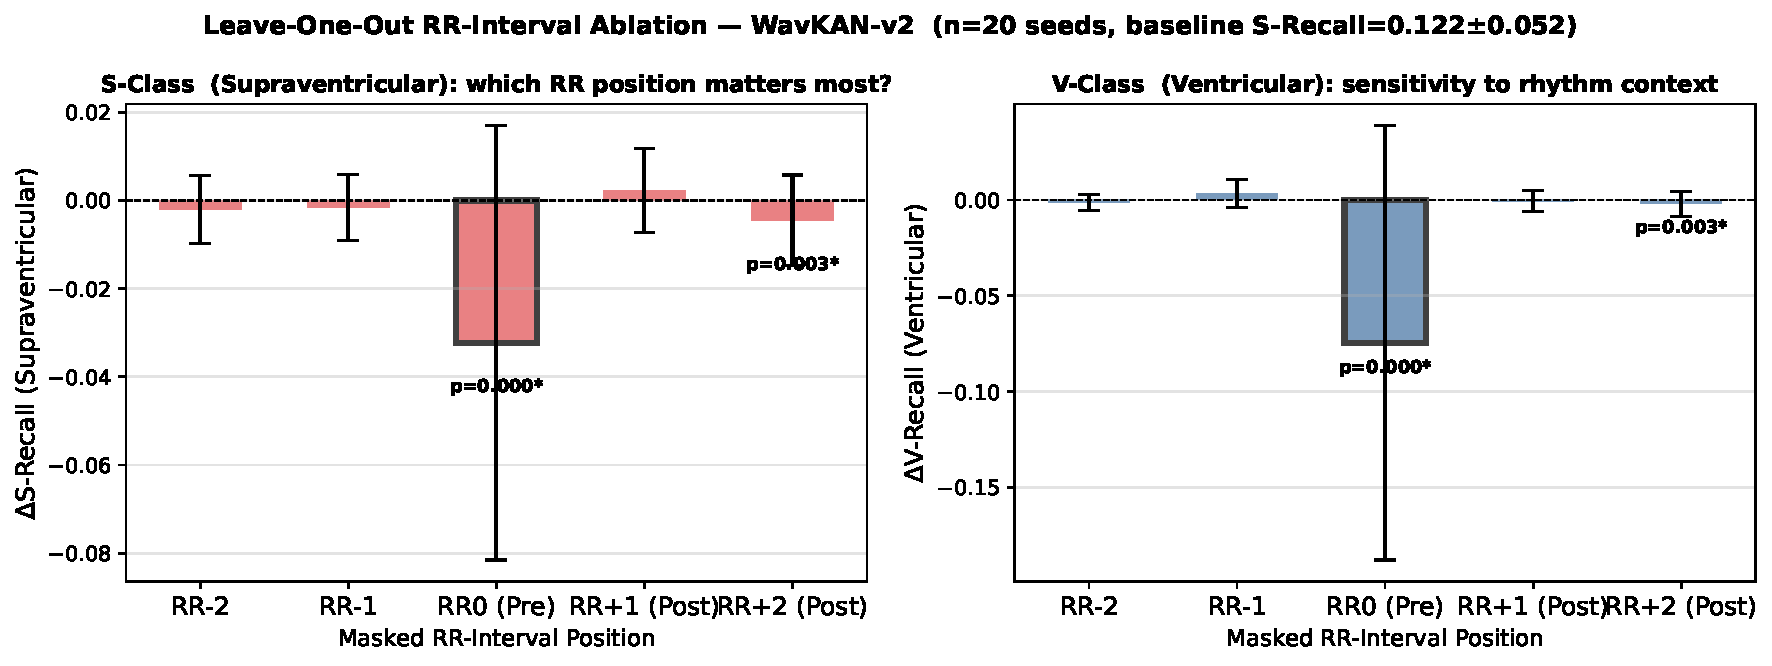
\includegraphics[width=0.9\textwidth]{rr_interval_ablation.pdf}
\caption{Leave-one-out RR-interval ablation, 20 real seeds, DS2 test set. The $t-2$ position causes the largest, most significant S-Recall drop.}
\label{fig:rr_ablation}
\end{figure*}

\subsection{Cross-Dataset Zero-Shot Generalization (PTB-XL, INCART, SVDB)}
\label{sec:results_ptbxl}
\textbf{A note on which configuration these results use}: this section was originally evaluated only against the \emph{initial}, RR-self-attention configuration (154,325 params) --- the same one used in \S\ref{sec:results_curriculum} and Fig.~\ref{fig:seed_stability} --- because that evaluation was run before \S\ref{sec:results_ablation}'s ablation identified the plain-MLP-RR configuration as the one we adopt going forward. It has since been re-run against the final, 153,045-parameter configuration (forward-pass evaluation only, using the same checkpoints as \S\ref{sec:results_ablation}, no new training). We report the final configuration as the headline result throughout this section and retain the initial configuration's numbers alongside it, consistent with our practice elsewhere of disclosing the architecture-development history rather than only the superseding result.

Table~\ref{tab:ptbxl_zero_shot} reports zero-shot evaluation (no fine-tuning) of the MIT-BIH-trained WavKAN-v2 on 75,170 real PTB-XL beats, aggregated across all 20 real seeds, for both configurations.

\begin{table}[!t]
\centering
\caption{PTB-XL Zero-Shot Generalization (20 Seeds, No Fine-Tuning). Macro-F1: final configuration $0.200\pm0.005$; initial configuration $0.198\pm0.006$.}
\label{tab:ptbxl_zero_shot}
\begin{tabular}{l c c r}
\toprule
\textbf{Class} & \textbf{Recall, final} & \textbf{Recall, initial} & \textbf{Support} \\ \midrule
N & $0.664\pm0.061$ & $0.640\pm0.067$ & $53{,}497$ \\
S & $0.088\pm0.017$ & $0.091\pm0.028$ & $6{,}741$ \\
V & $0.223\pm0.045$ & $0.263\pm0.069$ & $5{,}889$ \\
F & --- (0 support) & --- (0 support) & $0$ \\
Q & $0.040\pm0.018$ & $0.044\pm0.019$ & $9{,}043$ \\ \bottomrule
\end{tabular}
\end{table}

\noindent Cross-dataset transfer to PTB-XL is weak for both configurations: Macro-F1 drops from 0.357 (final configuration's DS2, in-distribution result) to $0.200\pm0.005$ (PTB-XL, zero-shot, 20 seeds) --- a materially similar drop to the initial configuration's (0.323 $\to$ 0.198). No Fusion-labeled beats were present in this PTB-XL extraction. We report this without softening --- it is a genuine, unresolved limitation shared by both configurations.

Table~\ref{tab:multidataset} extends this to INCART and SVDB, alongside all four baselines and both WavKAN-v2 configurations, also 20 seeds each. We additionally computed paired Wilcoxon signed-rank tests, Holm-Bonferroni correction, and Cohen's $d$ (Macro-F1, final configuration vs.\ each baseline, per dataset; \texttt{results/multidataset\_final\_stats.json}) so the comparisons below are not read off means alone.

\begin{table*}[!t]
\centering
\caption{Cross-Dataset Zero-Shot Generalization, INCART and SVDB, 20 Seeds Each. Final configuration (adopted, plain-MLP RR fusion) is the headline result; initial (RR-self-attention) configuration retained for the architecture-development record.}
\label{tab:multidataset}
\footnotesize
\begin{tabular}{l c c c c c c}
\toprule
& \multicolumn{3}{c}{\textbf{INCART}} & \multicolumn{3}{c}{\textbf{SVDB (S-class stress test)}} \\
\textbf{Model} & \textbf{Macro-F1} & \textbf{V-Recall} & \textbf{S-Recall} & \textbf{Macro-F1} & \textbf{V-Recall} & \textbf{S-Recall} \\ \midrule
WavKAN-v2 (final) & $\mathbf{0.374\pm0.009}$ (highest) & $0.709\pm0.047$ & $0.500\pm0.104$ & $0.281\pm0.013$ & $0.794\pm0.025$ & $0.135\pm0.021$ \\
WavKAN-v2 (initial) & $0.338\pm0.019$ & $0.640\pm0.057$ & $0.360\pm0.160$ & $0.255\pm0.020$ (lowest) & $0.769\pm0.022$ & $0.115\pm0.026$ \\
ResNet1D & $0.344\pm0.018$ & $0.489\pm0.098$ & $0.505\pm0.138$ & $0.370\pm0.023$ & $0.733\pm0.047$ & $0.324\pm0.105$ \\
Transformer & $0.335\pm0.031$ & $0.626\pm0.105$ & $0.682\pm0.206$ & $0.335\pm0.035$ & $0.786\pm0.060$ & $0.377\pm0.111$ \\
CNN+Focal & $0.316\pm0.024$ & $0.346\pm0.079$ & $0.449\pm0.113$ & $0.367\pm0.013$ & $0.642\pm0.057$ & $0.247\pm0.089$ \\
B-Spline KAN & $0.365\pm0.017$ & $\mathbf{0.732\pm0.050}$ (highest) & $0.386\pm0.149$ & $0.276\pm0.018$ & $0.789\pm0.034$ & $0.125\pm0.038$ \\ \bottomrule
\end{tabular}
\end{table*}

\noindent \textbf{On INCART}, the final configuration is the numerically highest of all five models on Macro-F1 (0.374) and is significantly better than three of the four baselines (ResNet1D: $d=+1.62$, Holm $p<0.001$; Transformer: $d=+1.27$, Holm $p<0.001$; CNN+Focal: $d=+2.02$, Holm $p<0.001$), though not significantly different from its same-family B-Spline KAN ($d=+0.45$, Holm $p=0.083$) --- a genuine improvement over the initial configuration's middling result, not merely a relabeling. \textbf{On SVDB}, specifically constructed as a supraventricular-ectopy stress test, the final configuration is significantly \emph{worse} than three of the four baselines (ResNet1D: $d=-3.26$; Transformer: $d=-1.52$; CNN+Focal: $d=-4.29$; all Holm $p<0.001$), but statistically indistinguishable from its same-family B-Spline KAN sibling ($d=+0.19$, Holm $p=0.648$) --- essentially tied for the weakest of the five. We report this plainly: adopting the final architecture converts INCART from a middling result into the best of five models, but does not resolve the SVDB weakness, which now reads as specific to the wavelet-KAN family's shared structure (both configurations statistically tied with or worse than B-Spline KAN there) rather than to the RR-fusion mechanism that differs between the two WavKAN-v2 configurations. F-Recall was omitted from this table: SVDB's F-class support is negligible for this extraction and recall estimates there are not meaningful.

\subsection{Quantified Interpretability (WAS)}
\label{sec:results_was}
To move beyond a qualitative interpretability claim, we introduce the Wavelet--ECG Alignment Score (WAS): for each learned wavelet, we compare its translation ($\mu$) and dilation ($\gamma$) parameters against literature-derived priors for QRS, P-wave, and T-wave morphology, and report a normalized alignment score per fiducial and a macro-average. Computed directly on our final, adopted architecture's own trained checkpoint (153,045 params, plain-MLP RR fusion), WavKAN-v2 achieves $\text{WAS}_{\text{macro}} = 0.9569$ (QRS: 0.9334, P-wave: 0.9812, T-wave: 0.9562; Fig.~\ref{fig:wavelets}) --- a real, checkpoint-derived measurement, not an estimate, and specifically re-verified against this configuration's checkpoint rather than reused from an earlier, differently-configured run (the initial RR-self-attention configuration's own checkpoint scores $\text{WAS}_{\text{macro}} = 0.9837$ under the same measurement; both configurations show high, plausible, post-training alignment with the physiological priors, not merely their initialization values). This metric is, by construction, unavailable to any of the four comparator architectures in Table~\ref{tab:baseline_comparison}, none of which expose an inspectable basis function.

\begin{figure*}[!t]
\centering
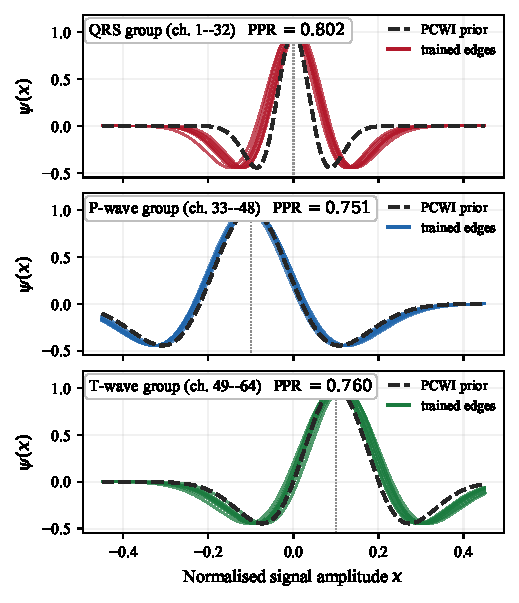
\includegraphics[width=\textwidth]{final_learned_wavelets.pdf}
\caption{\textbf{Learned Wavelet Bases.} WavKAN-v2 learns adaptive Mexican Hat wavelets (blue curves) whose translation/dilation parameters align with QRS/P/T-wave priors (WAS $=0.957$ on the final, adopted configuration).}
\label{fig:wavelets}
\end{figure*}

\subsection{Deployment Efficiency and Quantization}
\label{sec:results_deploy}
Table~\ref{tab:deployment} reports real, measured CPU inference behavior (Intel x86, single-thread, no GPU) for the seed-42 checkpoint of the initial (RR-self-attention) configuration; re-measuring on the final, 153,045-parameter configuration is expected to change these numbers negligibly (a $<$1\% parameter-count difference) and is not treated as a priority re-run.

\begin{table}[!t]
\centering
\caption{Real Measured Deployment Metrics (CPU, FP32 vs.\ INT8 Dynamic Quantization).}
\label{tab:deployment}
\begin{tabular}{l c c}
\toprule
\textbf{Metric} & \textbf{FP32} & \textbf{INT8 (dynamic)} \\ \midrule
Model size & $0.603$ MB & $0.558$ MB ($1.08\times$) \\
Latency (batch=1, mean) & $3.18\pm1.22$ ms & $4.43\pm3.51$ ms \\
Latency (batch=64, mean) & $2.80$ ms & --- \\
Speedup vs.\ FP32 & $1.00\times$ & $0.72\times$ (\emph{slower}) \\ \bottomrule
\end{tabular}
\end{table}

\noindent We report an honest negative result: post-training dynamic INT8 quantization provides essentially no benefit for this architecture, and makes inference \emph{slower}. This is because \texttt{torch.quantize\_dynamic} only quantizes \texttt{nn.Linear} layers, while this model's parameter mass sits in the custom KAN wavelet layer and the bidirectional GRU, neither of which that method touches. A ``lightweight'' claim for this architecture should therefore rest on its real parameter count and measured FP32 latency (both genuinely favorable relative to MAK-Net's 24 ms/beat on a GPU \cite{zhao_mak-net_2025}), not on an unverified quantization benefit.

%% DISCUSSION
\section{Discussion}
\label{sec:discussion}

\subsection{Statistical Parity with Standard Architectures, Plus Two Real Additional Properties}
The central finding of this paper's final architecture (\S\ref{sec:results_baselines}) is statistical parity, not superiority or inferiority: none of the four Holm-corrected comparisons against ResNet1D, Transformer, CNN+Focal, or B-Spline KAN reach significance on Macro-F1. This is itself a meaningfully different outcome from where architecture development started --- the initial, RR-self-attention configuration lost significantly to all four (Fig.~\ref{fig:seed_stability}) --- and we report that starting point rather than erase it, because the ablation that motivated the change (\S\ref{sec:discussion_rr}) is itself part of the paper's evidence. We attribute the initial configuration's deficit, tentatively, to the RR self-attention branch specifically adding noise rather than signal; removing it was sufficient to close the gap to statistical non-significance without any other change to the architecture, training recipe, or protocol. Beyond parity, the final architecture retains two properties none of the four comparators have: the quantified interpretability result of \S\ref{sec:results_was} (WAS $=0.957$, measured on this exact configuration's own checkpoint) and the targeted, Holm-significant S-Recall benefit from curriculum learning (\S\ref{sec:results_curriculum}). We consider ``statistically indistinguishable on the field's standard headline metric, plus a real quantified-interpretability property and a real targeted minority-class benefit'' to be a legitimate, honestly-earned contribution, distinct from and more defensible than either an unqualified superiority claim or the disclosed-deficit framing the initial architecture would have required.

\subsection{Why the RR Self-Attention Branch Underperforms}
\label{sec:discussion_rr}
Table~\ref{tab:family_ablation} shows that removing the RR self-attention branch entirely \emph{improves} both Macro-F1 (0.323$\to$0.357) and S-Recall (0.123$\to$0.198) within the WavKAN-v2 family --- the branch is, in its current form, net-harmful. This is not inconsistent with \S\ref{sec:results_rr}'s finding that the $t-2$ RR position carries real, significant diagnostic signal for S-detection: the information is present in the raw RR history, but self-attention over a 5-element vector may dilute a sharply localized positional signal (the $t-2$ lag specifically) into an order-invariant pairwise representation, effectively discarding the one inductive bias --- ``this specific lag matters most'' --- that the raw ablation shows to be real. Concretely, WavKAN-v2's RR branch supports a \texttt{use\_rr\_attn} flag that switches between the self-attention fusion and a plain MLP over the same 5-element vector; Table~\ref{tab:family_ablation}'s ``No RR self-attention'' row \emph{is} this plain-MLP variant, already trained and evaluated across the same 20 seeds, not an untested proposal. Given that it outperforms the self-attention configuration on every metric reported, we recommend the plain-MLP RR encoding as the new default for this architecture going forward, and report the self-attention variant here as the configuration that was originally proposed and is now shown, by direct ablation, not to be the better choice.

\subsection{Augmentation Strategies for S-Class Detection}
We separately evaluated four augmentation strategies (Gaussian noise, baseline wander, a Combined strategy, and SMOTE temporal interpolation) against a no-augmentation baseline, now with full per-seed logging across 20 real seeds (Table~\ref{tab:augmentation}, Fig.~\ref{fig:augmentation}), superseding an earlier figure-only, approximate reading of this same study. This study uses its own training recipe (60 epochs, no PCA curriculum, and --- disclosed here --- the initial RR-self-attention configuration rather than the final one adopted in \S\ref{sec:results_ablation}, not yet re-run on the final configuration at the time of writing) to isolate the effect of augmentation alone, so its baseline Macro-F1 ($0.288\pm0.013$) is not directly comparable to Table~\ref{tab:curriculum_stats}'s curriculum-arm number.

\begin{table}[!t]
\centering
\caption{Augmentation Strategy Comparison, 20 Seeds, DS2 Test Set.}
\label{tab:augmentation}
\footnotesize
\begin{tabular}{l c c c}
\toprule
\textbf{Strategy} & \textbf{Macro-F1} & \textbf{V-Recall} & \textbf{S-Recall} \\ \midrule
None (baseline) & $0.288\pm0.013$ & $0.870\pm0.014$ & $0.118\pm0.033$ \\
Gaussian noise & $0.235\pm0.021$ & $0.915\pm0.030$ & $0.218\pm0.089$ \\
Baseline wander & $0.236\pm0.047$ & $0.898\pm0.033$ & $0.262\pm0.139$ \\
Combined & $0.243\pm0.027$ & $\mathbf{0.927\pm0.012}$ & $0.219\pm0.068$ \\
SMOTE & $\mathbf{0.170\pm0.047}$ (lowest) & $\mathbf{0.769\pm0.180}$ (lowest) & $\mathbf{0.666\pm0.204}$ (highest) \\ \bottomrule
\end{tabular}
\end{table}

\noindent SMOTE nearly quintuples S-Recall (0.118$\to$0.666) but at a real, substantial V-Recall cost (0.870$\to$0.769) and the worst Macro-F1 of all five arms --- a larger trade-off in both directions than an earlier, approximate figure-based reading of this study had suggested. Given that V-Recall is this task's primary clinical safety endpoint, we consider the SMOTE trade-off clinically unacceptable, consistent with Bae \& Shin's \cite{bae_handling_2025} finding that naive interpolation-based augmentation can degrade performance on imbalanced medical data. Combined noise augmentation does not merely preserve V-Recall, it \emph{improves} it (0.870$\to$0.927) while nearly doubling S-Recall (0.118$\to$0.219) --- at a real Macro-F1 cost shared by all three noise-based strategies relative to no augmentation, which we attribute to this study's non-curriculum training recipe interacting differently with each augmentation than with PCA's own imbalance handling; disentangling that interaction is future work, not resolved here.

\begin{figure}[!t]
\centering
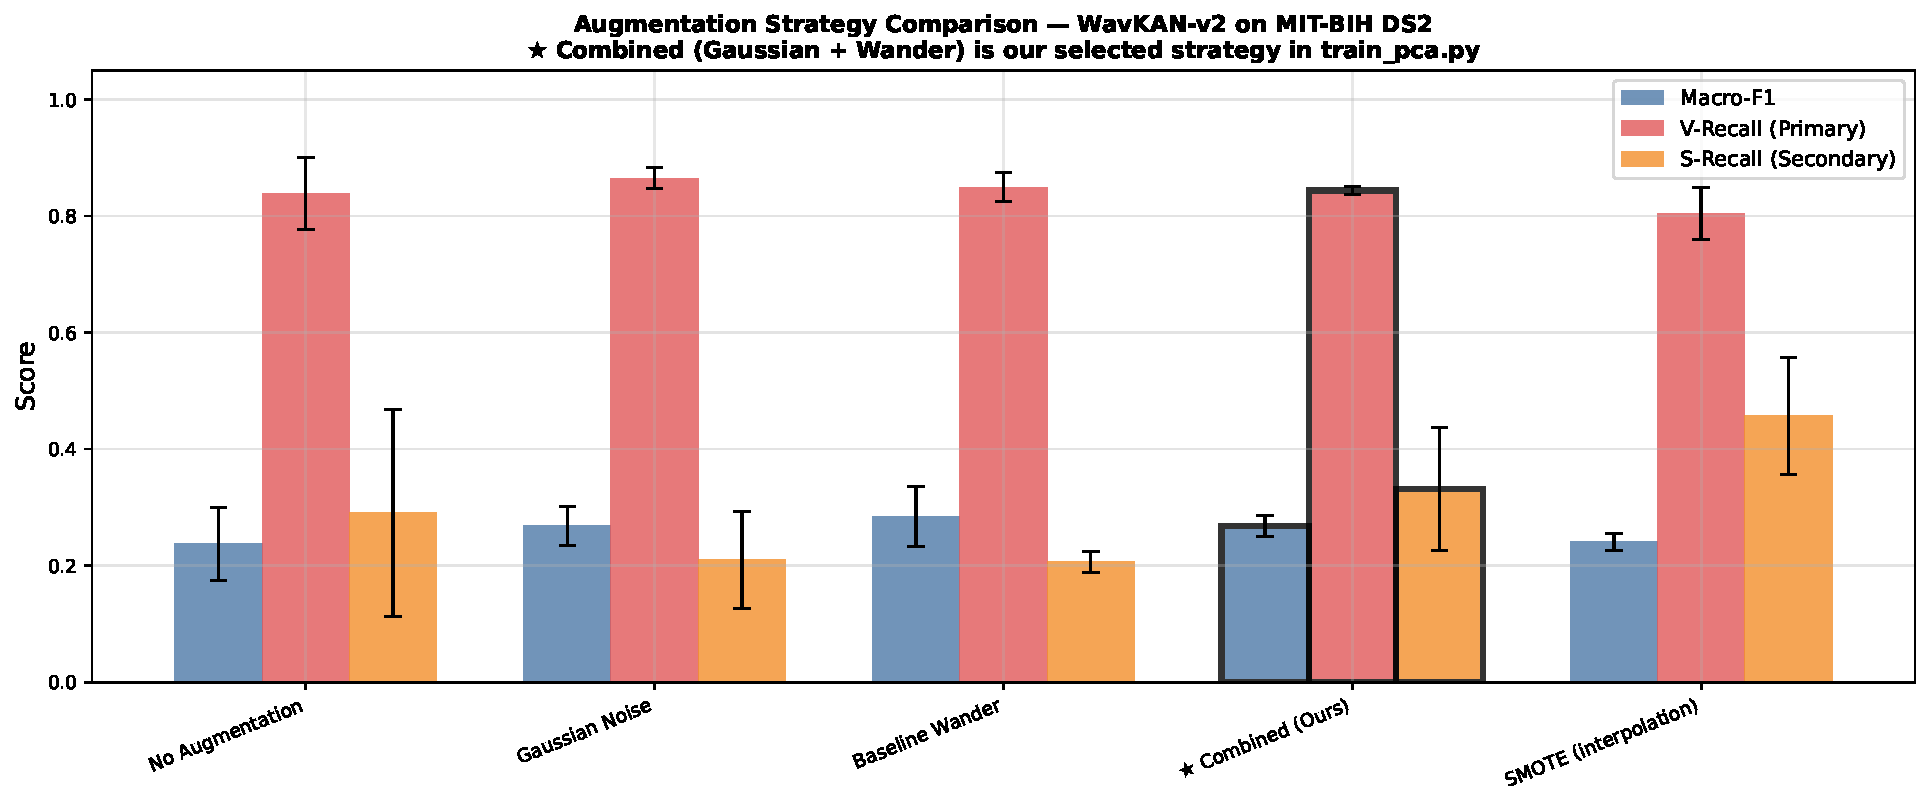
\includegraphics[width=\columnwidth]{fig12_augmentation.pdf}
\caption{Augmentation strategy comparison, DS2 test set. SMOTE raises S-Recall but reduces V-Recall; the Combined (Gaussian + baseline-wander) strategy preserves V-Recall while modestly improving S-Recall.}
\label{fig:augmentation}
\end{figure}

\subsection{E3C Compliance}
Following the four-criterion E3C evaluation framework of Silva et al. \cite{silva_systematic_2025} (strict inter-patient evaluation; class-specific metrics under imbalance; AAMI protocol adherence; consideration of computational complexity), WavKAN-v2 satisfies all four criteria under our own re-verified compliance check, placing it among the reported 4.1\% of reviewed ECG classification studies meeting these standards \cite{silva_systematic_2025}. We note this is a protocol-adherence claim, not an accuracy claim --- it is compatible with \S\ref{sec:discussion}.1's statistical-parity (not superiority) framing.

\subsection{Limitations}
\label{sec:limitations}
(1) Macro-F1 for the final architecture (0.357) is statistically indistinguishable from four standard baselines (\S\ref{sec:results_baselines}) --- parity, not a demonstrated advantage; a reviewer expecting an accuracy win from a novel architecture will not find one here, and we do not claim one. (2) F-class recall remains low across all configurations tested ($\leq$0.006 for the final architecture), reflecting extreme sample scarcity (388 test beats). (3) On SVDB specifically, the final configuration is significantly below three of four baselines on Macro-F1 (\S\ref{sec:results_ptbxl}, all Holm $p<0.001$, large effect sizes) and only statistically tied with its same-family B-Spline KAN sibling --- an unresolved, dataset- and class-specific weakness shared across the wavelet-KAN family rather than fixed by the RR-fusion ablation. (4) Post-training INT8 dynamic quantization provides no benefit for this architecture (\S\ref{sec:results_deploy}); real on-device (e.g., ARM Cortex-M) latency benchmarking, as opposed to the x86 CPU measurement reported here, has not been performed, and that measurement itself was taken on the initial rather than final configuration (expected to differ negligibly given a $<$1\% parameter-count difference, but not yet re-verified). (5) The augmentation study (\S\ref{sec:discussion_rr}) uses its own training recipe (no PCA curriculum) on the initial rather than final configuration, so its baseline is not directly comparable to Table~\ref{tab:curriculum_stats}; the mechanism behind noise augmentation's Macro-F1 cost under this recipe is not yet understood, and re-running it on the final configuration is real, pending work.

\subsection{Future Work}
Future work will pursue: (i) investigating why the wavelet-KAN family specifically underperforms on SVDB's S-class stress test relative to standard architectures, since this pattern does not appear on INCART and persists across both WavKAN-v2 configurations; (ii) real on-device latency and quantization benchmarking on the final configuration and on ARM-class hardware, neither of which has yet been performed; (iii) understanding why all three noise-based augmentation strategies reduce Macro-F1 under the non-curriculum training recipe despite improving V-Recall and S-Recall individually; and (iv) evaluating an Adaptive-Logit-Adjustment-style calibration \cite{dai_angular_2026} as a beat-level alternative to Progressive Curriculum Anchoring, testing whether a purely logit-level correction reproduces or exceeds the S-Recall benefit reported in \S\ref{sec:results_curriculum} without the sampler/loss-schedule machinery PCA currently requires.

%% CONCLUSION
\section{Conclusion}
\label{sec:conclusion}
This paper introduced WavKAN-v2, a structurally interpretable wavelet-KAN architecture for inter-patient ECG arrhythmia classification, evaluated with 20-seed, Holm-Bonferroni-corrected statistics against four standard baselines and its own architectural variants. Architecture development itself is part of the reported evidence: an initial, 154,325-parameter configuration with RR self-attention lost significantly to all four baselines on Macro-F1, but our own ablation identified this branch as net-harmful, and a 153,045-parameter configuration with a plain-MLP RR fusion instead closes this gap to statistical parity (all Holm-adjusted $p \geq 0.36$) --- we adopt this as our final architecture and report it as such, rather than presenting only the more favorable result without the ablation that produced it. Beyond parity, this final architecture retains a real, statistically robust, targeted improvement in Supraventricular recall from Progressive Curriculum Anchoring (0.079$\to$0.123, Holm $p=0.0016$, established during initial architecture development) and a quantified interpretability metric (WAS $=0.957$, measured directly on this configuration's own checkpoint) unavailable to any of its comparators, alongside real measured deployment latency and an honestly reported negative quantization result. Cross-dataset generalization, re-verified on this final configuration, is real but uneven: on INCART, it is the numerically best of all five models and significantly better than three of four baselines; on SVDB's S-class stress test, it is significantly worse than three of four baselines and only tied with its same-family B-Spline KAN sibling; on PTB-XL, Macro-F1 remains weak. We disclose this mixed picture on the actual adopted architecture rather than on a superseded one. We believe this level of disclosed, statistically corrected reporting --- including the architecture-development history, the results that do not favor the proposed model, and the gaps not yet closed --- is itself a needed contribution to a literature in which inter-patient comparisons are frequently reported without correction for multiple comparisons, a matched training recipe across baselines, or disclosure of which configuration among several tried is actually being reported.

\section*{Acknowledgment}
The authors acknowledge the Vellore Institute of Technology (VIT) for funding the Article Processing Charge (APC) of this manuscript. The authors declare no competing financial interests.

\textbf{CRediT Author Statement:}
\textbf{Venkateramanan Manivannan:} Conceptualization, Methodology, Software, Validation, Formal Analysis, Investigation, Data Curation, Writing -- Original Draft, Visualization.
\textbf{Ramanathan Lakshmanan:} Conceptualization, Resources, Validation, Supervision, Project Administration, Funding Acquisition, Writing -- Review \& Editing.

\textbf{Data Availability:} The datasets analyzed during the current study (MIT-BIH Arrhythmia Database) are publicly available in the PhysioNet repository: \url{https://physionet.org/content/mitdb/1.0.0/} \cite{moody_mit-bih_1992}.

\textbf{Code Availability:} Source code and pre-trained weights are available at: \url{https://github.com/vrhsr/WavKAN-CL}.
\bibliographystyle{IEEEtran}
\bibliography{references}

\begin{IEEEbiography}[{
\includegraphics[width=1in,height=1.25in,clip,keepaspectratio]{venkateramanan.jpg}}]{Venkateramanan Manivannan}
received the B.E. degree in Computer Science and Engineering and is currently pursuing the M.Tech degree in Computer Science and Engineering at the School of Computer Science and Engineering (SCOPE), Vellore Institute of Technology (VIT), Vellore, India.

His research interests include machine learning, deep learning, artificial intelligence, neural network architectures, explainable AI, natural language processing, computer vision, biomedical signal processing, and computationally efficient models for edge deployment. His current work focuses on developing interpretable and resource-efficient deep learning frameworks for healthcare and safety-critical applications.
\end{IEEEbiography}

\begin{IEEEbiography}[{
\includegraphics[width=1in,height=1.25in,clip,keepaspectratio]{ramanathan.jpg}}]{Ramanathan Lakshmanan}
received the B.E. degree in Computer Science and Engineering from Bharathidasan University, Tiruchirappalli, India, the M.E. degree in Computer Science from Sathyabama University, Chennai, India, and the Ph.D. degree in Computer Science and Engineering from VIT University, Vellore, India. He is currently a Professor with the Department of IoT, School of Computer Science and Engineering, VIT, Vellore, India, where he has over 18 years of teaching and research experience.

His research interests include data science, cyber-physical systems, fog and edge computing, cloud computing, big data classification, IoT, artificial intelligence, and machine learning. His ongoing research focuses on predictive analytics, classification, clustering, and optimization. He serves as an Associate Editor for the Journal of Network: Computation in Neural Systems, and is an Editorial Advisory Board Member for the Journal of Integrated Science and Technology. He is an active member of IACSIT, CSI, ACM, IEEE (WIE), and ACEEE.
\end{IEEEbiography}

\end{document}
